\section{Common ship body and propulsion types}

Throughout history, countless ship types have been brought to life, due to the various and ever-changing environmental challenges they had to overcome. Therefore they can be grouped or ordered several different ways, based on their shape, propulsion, area of application, origin and so forth. Modern ships have introduced remarkably advanced or creative propulsion technologies, Sky-sails resembling huge parachutes\cite[p 48.]{future_propulsions} that can be retrofitted to every ship, and even more are still in development, like the Magnetohydrodynamic propulsion\cite[p. 61.]{future_propulsions}. This section will give a quick overview about the most widespread possibilities, but the thesis will analyze only some of them.

\subsection{Hull types}

The lore of shipbuilding\footnote{Just like many other scholars of ancient history, early masters of shipbuilding were considered artists \cite{Art_of_shipbuilding}} is centered around the design of the hull, and it's probably a sensible way to start categorizing ships.
The fundamental concept of a ship hull design is the low resistance along the direction of forward motion. A lower drag results in faster top speed and lower energy requirements. Lateral shape is only mildly important in the design of self propelled ships, however sailing with a steep angle to the wind is only possible by balancing the front and lateral resistances carefully\cite{vitorlazas}.

\paragraph{Lateral surface} affects the ability of the ship to sail and turn. Large lateral surface results in good wind-response but generally decreases the turning agility and often increases the frontal surface and friction.

\subsection{Stability of a ship}

Stability is the ability of the vessel to return to it's previous position\cite{stability}. This righting movement is the result of the relationship between the \textbf{Center of Mass} (CoG), and the \textbf{Center of Buoyancy} (CoB) of the ship. The stability can be divided to three different movements, independent from each other.

\paragraph{Static stability} is the stability at rest, without any external forces. In contrary to the CG, which is a point fixed to the body of the ship\footnote{Unless the ship features moving ballast, like the sailor of a dinghy}, the CoG constantly changes it's position as the ship heels or trims. If the CoB and CoG don't align vertically, the ship keeps changing it's attitude, until they do.

\begin{figure}[H]
	\centering
	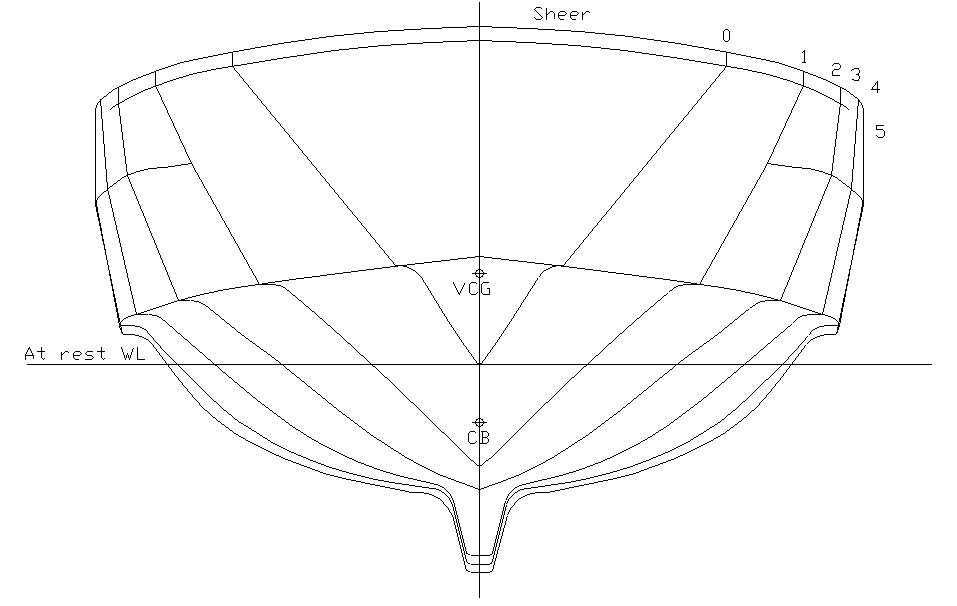
\includegraphics[width=0.6\textwidth]{img3/stability0}
	\caption{Static stability of a still boat\\http://www.brayyachtdesign.bc.ca/}
	\label{fig:stability0}
\end{figure}

\paragraph{Form stability} As the boat moves, some area submerges, some reveals from the water. As the hull is heeling, the CoB moves, and depending on the form stability the boat will either overturn, or enough counter-tourqe will build up to reverse the tilting motion.

\begin{figure}[H]
	\centering
	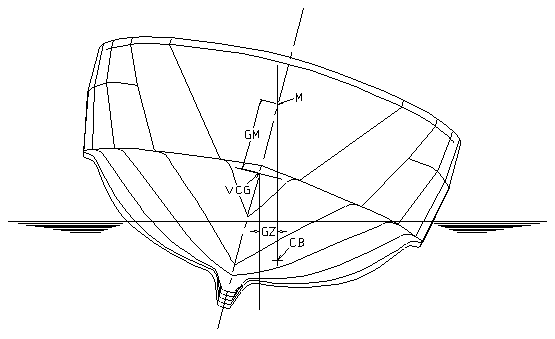
\includegraphics[width=0.6\textwidth]{img3/stability1}
	\caption{Form stability of a heeling boat\\http://www.brayyachtdesign.bc.ca/}
	\label{fig:stability1}
\end{figure}

\paragraph{Dynamic stability} is generated when the ship is moving, and the effect is increased with speed. The dynamic stability can either increase or decrease the overall stability, but most modern boats are considerably more stable at higher speeds, due to special hull shaping. As the pressure increases under the hull, the dynamic forces will become stronger compared to the effects of buoyancy, and a round-bottomed hull can become unstable, as the width and shape of the hull beneath the water is significantly narrower than during static buoyancy.

\begin{figure}[H]
	\centering
	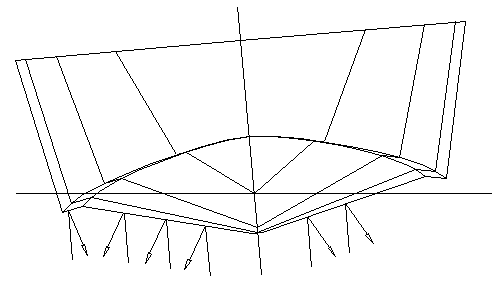
\includegraphics[width=0.6\textwidth]{img3/stability2}
	\caption{Dynamic stability of a speeding boat\\http://www.brayyachtdesign.bc.ca/}
	\label{fig:stability2}
\end{figure}

\paragraph{Stability in general} It's notable, that even though a boat with high form and dynamic stability can offer a pleasant still water comfort, also provides a very rough ride at higher speeds, due to the quick hull reactions. On the contrary, a smooth wave-cutter promises constant swaying and vertical movement in a harbor.

One of the earliest efforts to increase stability was the extra \textbf{Ballast} added to the bottom of the ship, ranging from a couple of rocks to a keel mounted metal fin. The principle of the ballast is to lower the center of gravity. Many modern sailboats feature a lower CoG than the CoB therefore becoming immune to capsizing. Even after a complete turnover, the boat will eventually return to it's original state\footnote{Given that no structural damage happened during this undesirable event}.
Another, but considerably different effort to ensure stability is a wide \textbf{Beam}ed hull. While the ballast provides good ultimate stability, it lacks the initial stability, and the body can gather up quite some tilt until the gravity starts working. Contrary to the ballast, a wide beam provides good initial stability but does not provide the righting movement after a certain point. However,  wide beam monohulls can be dangerous, because it reaches the peak of initial stability quickly and the ship is more likely to capsize, but multihulls\footnote{Catamarans, trimarans} can boast exceptional stability qualities.

\begin{figure}[H]
	\centering
	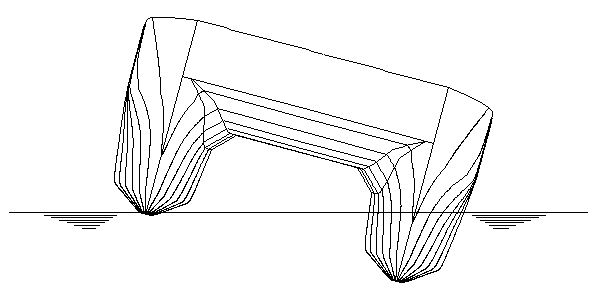
\includegraphics[width=0.6\textwidth]{img3/stability3}
	\caption{Wide beam multihull boat\\http://www.brayyachtdesign.bc.ca/}
	\label{fig:stability3}
\end{figure}

The response speed of the ship can be adjusted by the placement of equipment and cargo on the ship. By moving weight away from the centerline horizontally, the increased \textbf{inertia} dampens the quick movements caused by high initial stability. If a ship is close to turning over completely, a well-designed \textbf{Superstructure} can still have a positive impact on the stability, and save the day. Unfortunately, a large superstructure is effected by heavy winds, which can be a problem, if the ship lacks a good stability.

In conclusion, adequate stability can be ensured with common sense during the design process, but an all round stability is the result of careful planning.

\paragraph{Sailing rigg} 

Many centuries had to pass until humanity discovered the way to sail sideways to the wind, and even towards the wind in some degree. Modern sailboats still provide a good alternative to motorised ships especially in still water. Contrary to the belief, sailing ships are not the only wind powered ships currently existing, although they proved to be the most efficient. However, Rotor ships are still manufactured\cite[p. 47.]{future_propulsions}, mostly as part of a hybrid propulsion system.

Wrapfig Here.

Regulations in the European Union even prevent the usage of petrol engine in Lakes unless sailing in the harbour or under hazardous conditions, and sailboats are still popular for recreational use. The sails, the mast, the ropes and other similar equipment are all part of the rig. The rigging has many various forms depending on the number of masts, size of the ship and the type of sails. The most widespread type of modern and sailing yachts is the single masted rig with two triangular sails. The fore-sail  is fixed while the mainsail can be rotated with the boom. There are a lot of additional sail types, especially on the racing boats. Most common of them is the spinnaker, which is a large parabolic sail used for reaching, often featuring colorful graphics.

Wrapfig:
To see a long boomed gaffer overtaking from dead upwind with spinnaker on one side, and main, topsail and watersail on the other, is devastating. She seems to fill the sky, while the air for 50yds ahead of her is so still that the victim's pipe-smoke goes straight up as his yacht is inexorably overhauled.
—Cunliffe, Tom, (1992). Hand, Reef and Steer, Adlard Coles Nautical, London

\paragraph{Mechanized propeller propulsion}

Every ship, even before the steam engine was invented featured some sort of mechanical propulsion, most notably rowing galleys. Modern yachts offer petrol or electric engines instead. In case of smaller boats the drive train consists of a shaft connected to the engine, a propeller and a rudder. Jet propulsion, which only the fastest sports and jetskis feature is less common, because they sacrifice efficiency for speed.
Large ships and submarines are often outfitted width a nuclear power plant, although for different reasons. In case of large vessels the primary motivation is the almost unlimited range, because a nuclear reactor can provide enough power to keep the ship on the sea for a very long time, and the replenishment of fuel has become only a small nuisance\cite[nuclear_range].On the contrary the primary advantage of the nuclear engines in a submarine is the fact that it doesn't require air for the power production process. The underwater range of early submarines were limited because they had to emerge from time to time to the surface where they are exposed to detection and enemy fire\cite[nuclear_submarine].

\subsection{Design conclusions}

In case of a civilian unmanned surface vehicle many problems described above can be ignored because of the small size of the boat, the lack of human crew and non-military application.
Stability is very important in case of sailing vessels, because stronger wind can create a large torque on the ship. Single and multihull vessels respond to this torque entirely differently. The single hull boat is stabilised by a keel mounted ballast that provides low initial stability, the boat will heel and the effective sail size will reduce, but ultimately will remain stable thanks to the reserve stability. On the contrary, a multi-hull ship featuring high initial stability will respond with rapidly increasing speed. This characteristic has made catamarans and especially trimarans very popular among racers, but they carry the dangers of tripping over. And the righting of a capsized trimaran is hardly possible without external help. In conclusion, a  trimaran can easily outperform a classic sailboat in terms of speed and agility, but they can be used safely in a controlled environment only. On the other hand a single-hull boat with a weighted keel and sufficiently watertight inner compartments is much more reliable in the harsh environment of an ocean.

During the thesis two different ships types will be designed. The first vessel is a short range electric motorised boat, featuring a multi-hull trimaran design. Primary application areas are short missions requiring high speed, agility and quick mobilisation. The ship class has been named after a small but agile carnivorous bird: the Kestrel.

The second is a single-hull sailboat capable of conducting long-range measurements where regular maintenance is impossible and high reliability must be ensured. This ship class was named after the iconic bird of long annual travel: the Stork.

[Table comparing the pros and cons of the designs]